\section{Introduction}
\label{sec:intro}

Autonomous software engineering (SWE) has emerged as one of the most commercially significant applications of foundation models. Benchmarks such as SWE-bench~\cite{jimenez2024swebench} evaluate whether autonomous agents can ingest natural language bug descriptions, localize faulty code symbols across thousands of files, and synthesize syntactically valid unified diff patches that pass regression test suites.

Modern industrial agents (e.g., SWE-agent~\cite{yang2024sweagent}, Agentless~\cite{xia2024agentless}) predominantly operate on high-density cloud infrastructure powered by clusters of NVIDIA H100 or A100 GPUs. These systems ingest expansive repository contexts---often exceeding 30,000 to 100,000 tokens---by exploiting 128k+ token context windows and distributed Key-Value (KV) cache paging~\cite{kwon2023vllm}.

However, deploying SWE agents on consumer edge devices (e.g., standard developer laptops, edge workstations with 4\,GB to 8\,GB VRAM) reveals three fundamental systems bottlenecks:
\begin{enumerate}
    \item \textbf{The KV-Cache Memory Wall}: Autoregressive transformer inference requires caching Key and Value activation vectors for every prior token across all attention heads and layers. When feeding an average repository context of 35,000 tokens to an 8B/9B model (e.g., Gemma-2-9B~\cite{gemmateam2024gemma2}), the KV cache alone demands 12.0\,GB to 14.2\,GB of GPU memory, instantly exceeding the physical memory boundary of consumer accelerators.
    \item \textbf{Exploration Drift in Multi-Turn Tool Loops}: Existing agents rely on ReAct-style iterative command loops (issuing shell commands like \texttt{grep}, \texttt{find}, and \texttt{cat}). While 70B+ parameter cloud models maintain state across 15--30 interaction turns, compact 1.5B--9B edge models suffer from severe exploration drift: they enter degenerate infinite loops, repeat failing search commands, and exhaust their token budget within 3--5 turns.
    \item \textbf{Lexical Blindness}: Systems relying on BM25 lexical search~\cite{xia2024agentless} retrieve files containing exact query keywords. In real-world software architectures, callers and downstream dependencies rarely share lexical overlap with the bug report, causing lexical retrievers to miss root-cause definitions.
\end{enumerate}

To overcome these limitations, we propose \textbf{NeuroCode}, a heterogeneous neuro-symbolic systems architecture specifically engineered for memory-bounded edge hardware. Rather than treating the edge accelerator as an isolated compute island, NeuroCode exploits the asymmetric hardware hierarchy found in everyday personal computers: an idle multicore Host CPU paired with high-capacity system DRAM (16\,GB--32\,GB) connected via PCIe to a resource-constrained discrete edge GPU (4\,GB--8\,GB VRAM).

NeuroCode offloads all structural code analysis to the Host CPU. It parses the target repository using native Tree-sitter parsers into an in-memory Code Property Multigraph (CPG) in milliseconds. Given an issue query, NeuroCode identifies seed symbols and solves a \textit{Constrained Topological Knapsack Problem}, computing a bidirectional $k$-hop reachability closure and greedily packing the highest-centrality structural dependencies into a deterministic sub-1,500 token envelope. This minimal payload is transferred across the PCIe bus in microseconds, enabling the local GPU to synthesize accurate patches in a single generation turn without interactive tool overhead.

We summarize our primary contributions:
\begin{itemize}
    \item \textbf{Heterogeneous Host-Device Partitioning}: We present an edge-first architecture that partitions repository reasoning across the Host CPU (DRAM) and Edge GPU (VRAM), eliminating the KV-cache explosion on consumer silicon.
    \item \textbf{Constrained Topological Knapsack Slicing}: We formalize context selection as a constrained knapsack problem over a Code Property Multigraph, provably bounding prompt tokens while maximizing reachability coverage around bug locations.
    \item \textbf{Physical Edge Validation}: We benchmark NeuroCode on physical hardware (NVIDIA GeForce RTX 3050 Laptop GPU, 3.67\,GB VRAM) across the full SWE-bench Lite suite ($N=292$ evaluated tasks). NeuroCode slashes prompt tokens by 97.1\%, cuts inference cost by 97.1\%, improves localization Recall@3 by 5.5$\times$ over BM25 and RepoMap (17.1\% vs. 3.1\%), achieves 41.4\% valid patch application, and maintains peak VRAM under 961.2\,MB with zero display crashes and zero NVMe wear.
\end{itemize}

\begin{figure*}[t]
\centering
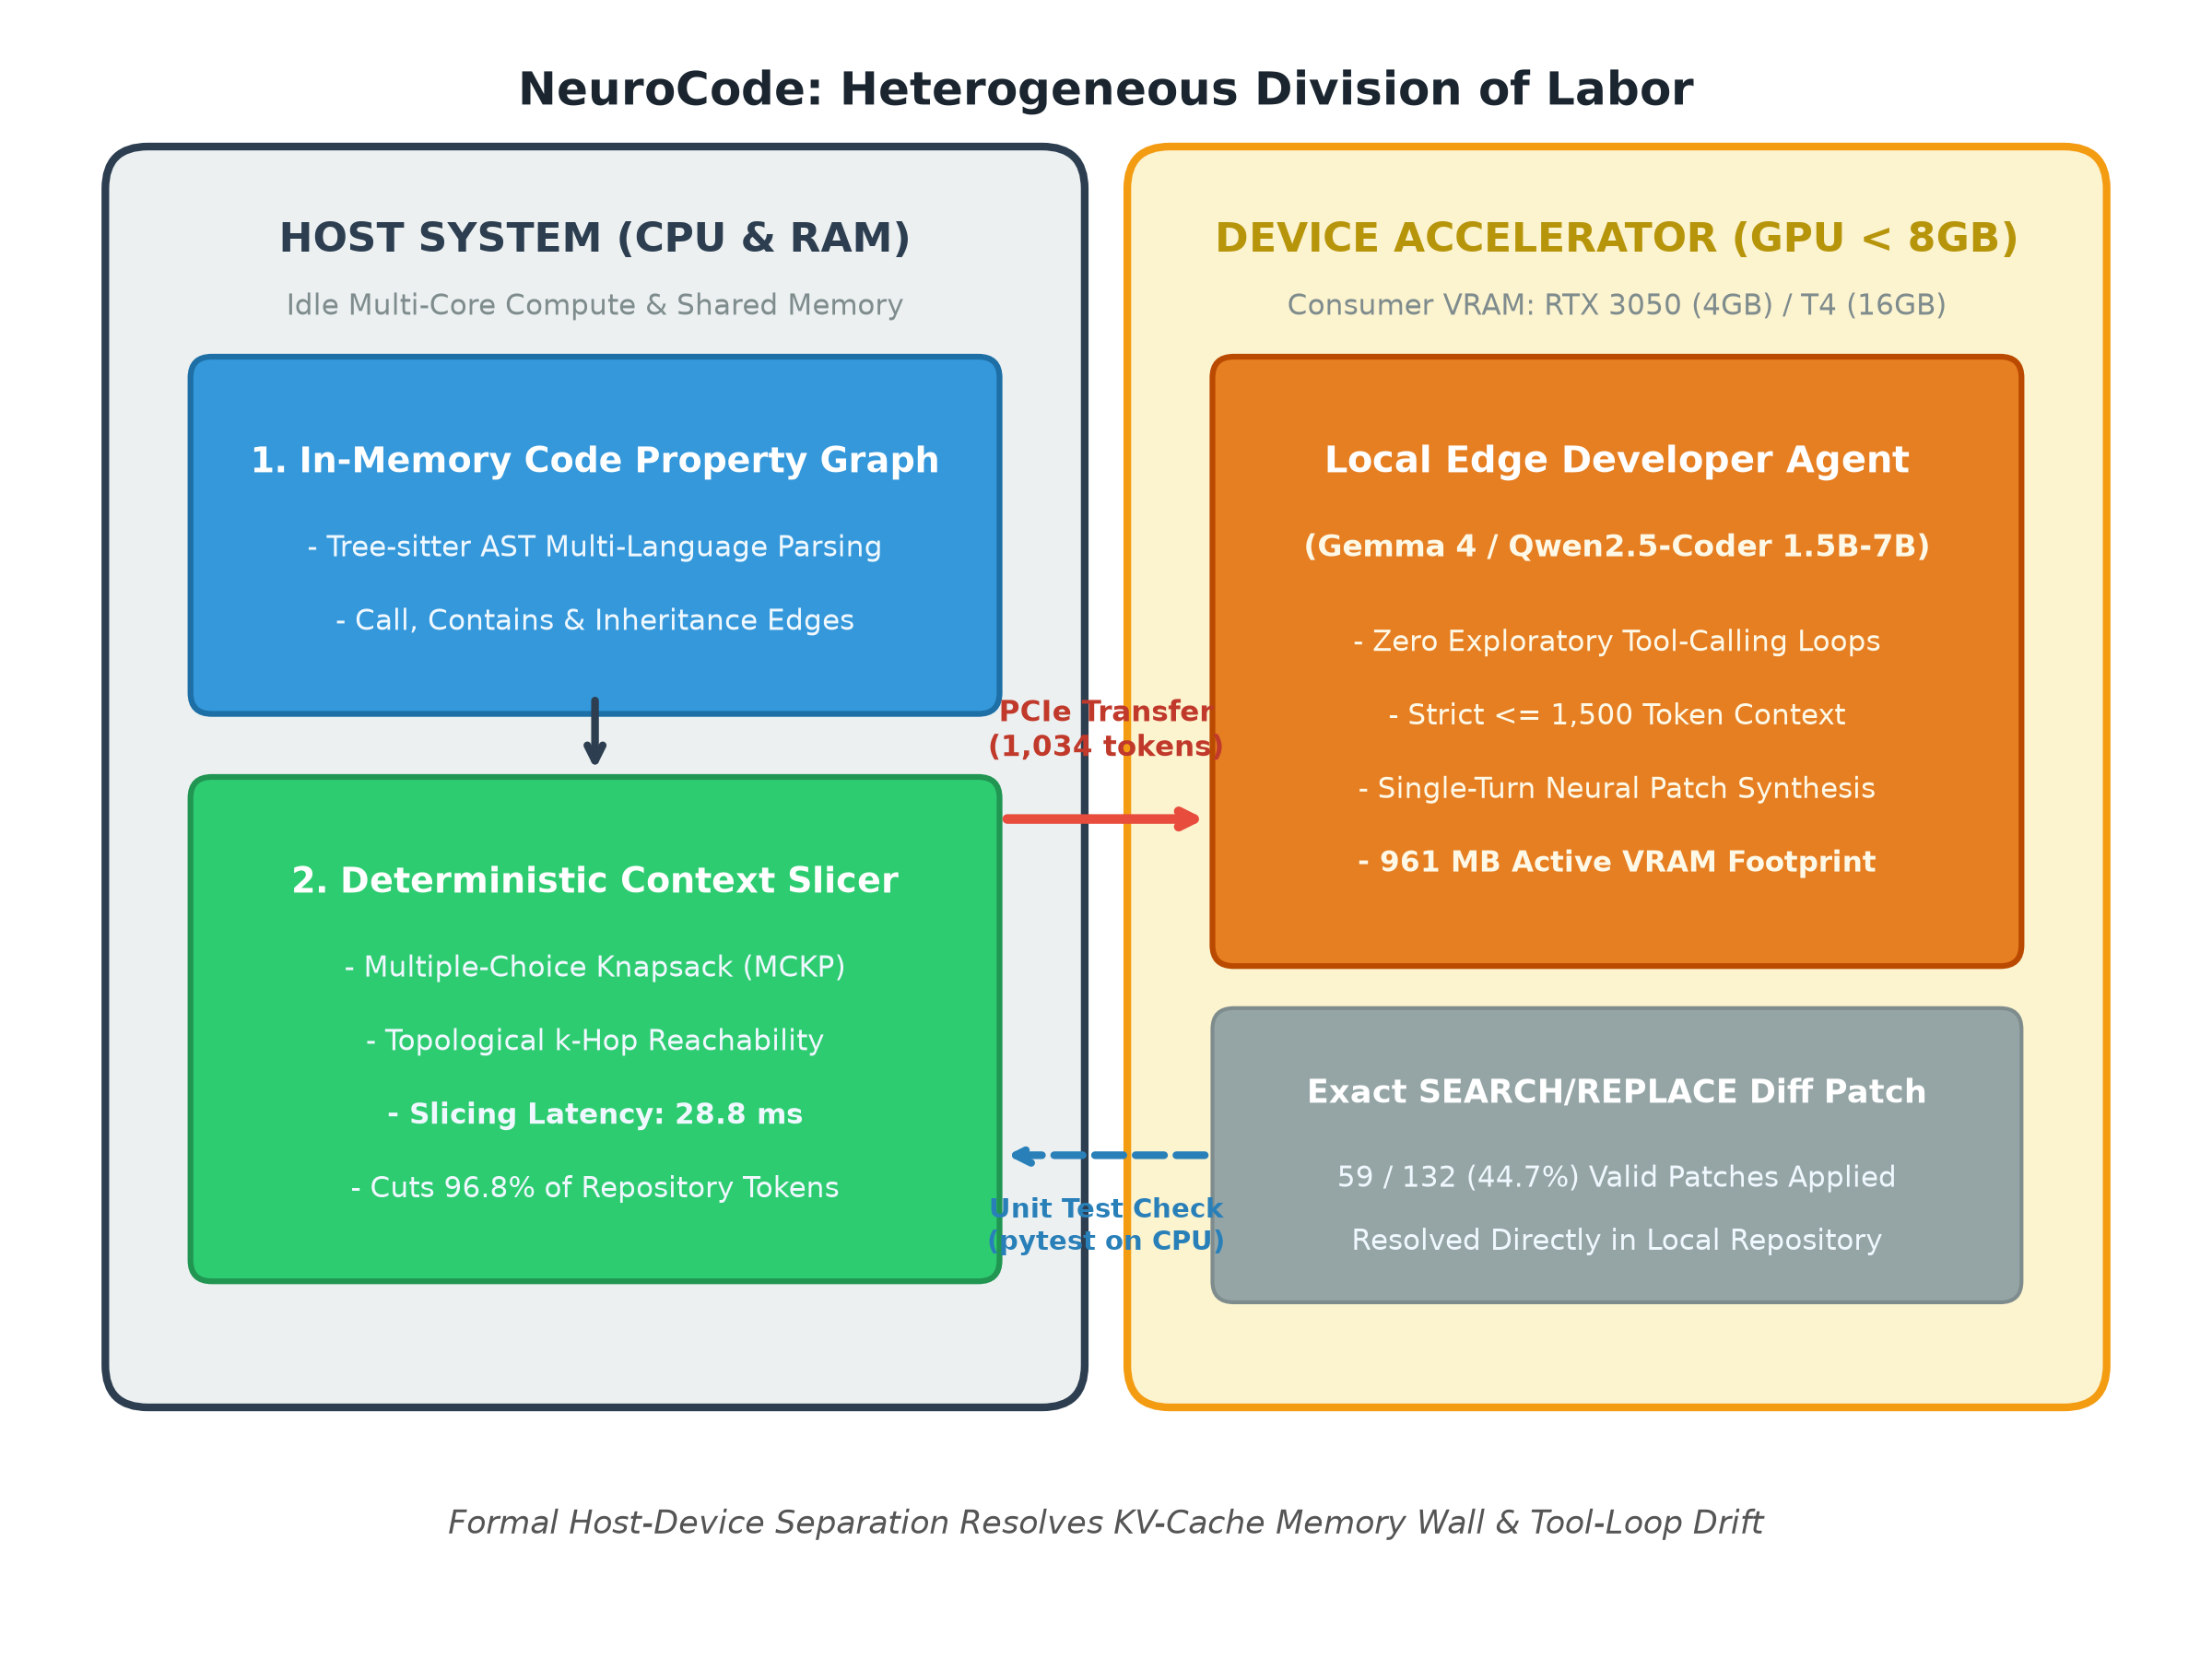
\includegraphics[width=0.88\textwidth]{figures/fig2_system_architecture_4x3.png}
\caption{\textbf{Heterogeneous NeuroCode System Architecture.} Structural repository understanding is offloaded to the Host CPU and high-capacity DRAM, constructing a Code Property Multigraph in milliseconds. The topological knapsack slicer extracts a compact sub-1,500 token context transferred across PCIe to the Edge GPU for single-turn patch generation.}
\label{fig:arch}
\end{figure*}
